\subsection{Structured Data}

\subsubsection{Definition of Structured Data}
\begin{frame}{Definition of Structured Data}
Within the scope of this lectures, structured data or a table is a sequence of tuples
\begin{itemize}
    \item Each tuple is a data point with features
    \item Not all data points have the same set of features
\end{itemize}

\end{frame}

\begin{frame}{Example}
    \begin{center}
    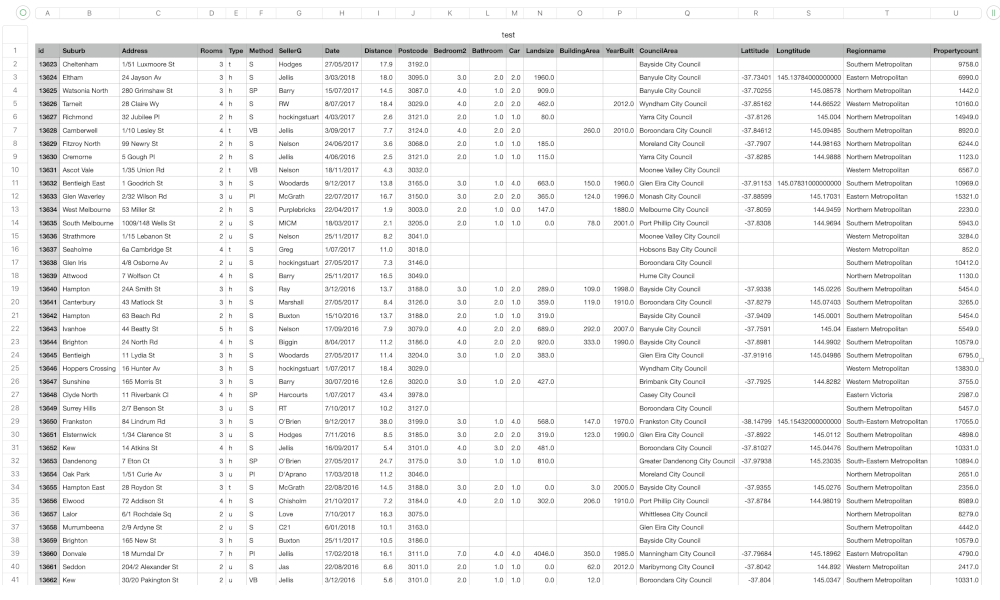
\includegraphics[width=\textwidth]{assets/defintion_structured_data.png}
    \end{center}
\end{frame}

\subsubsection{Data Cleaning}

\begin{frame}{Data Cleaning - Motivation}

Structure data in real world are not perfect. There might be

\begin{itemize}
    \item Incomplete data / missing values
    \item Noisy data
    \item Inconsistent data
\end{itemize}

\end{frame}

\begin{frame}{Data Cleaning - Missing Values}

Several tuples might not have all the features. In that case, we can

\begin{itemize}
\item Remove the tuples
\item Manually fill in missing values \\
by measure of central tendency (mean, median) \\ 
by measure of central tendency with class label \\ 
by prediction model \\
\end{itemize}
\end{frame}

\begin{frame}{Data Cleaning - Noise}

There might be noise in data. Noise is random and independent with data.
\begin{exampleblock}{Additive Noise}
    \begin{equation}
        x^{*} = x + z
    \end{equation}
    where $x \sim X$ and $z \sim Z$ such that $Z$ is i.i.d with itself and $X$
\end{exampleblock}
\begin{center}
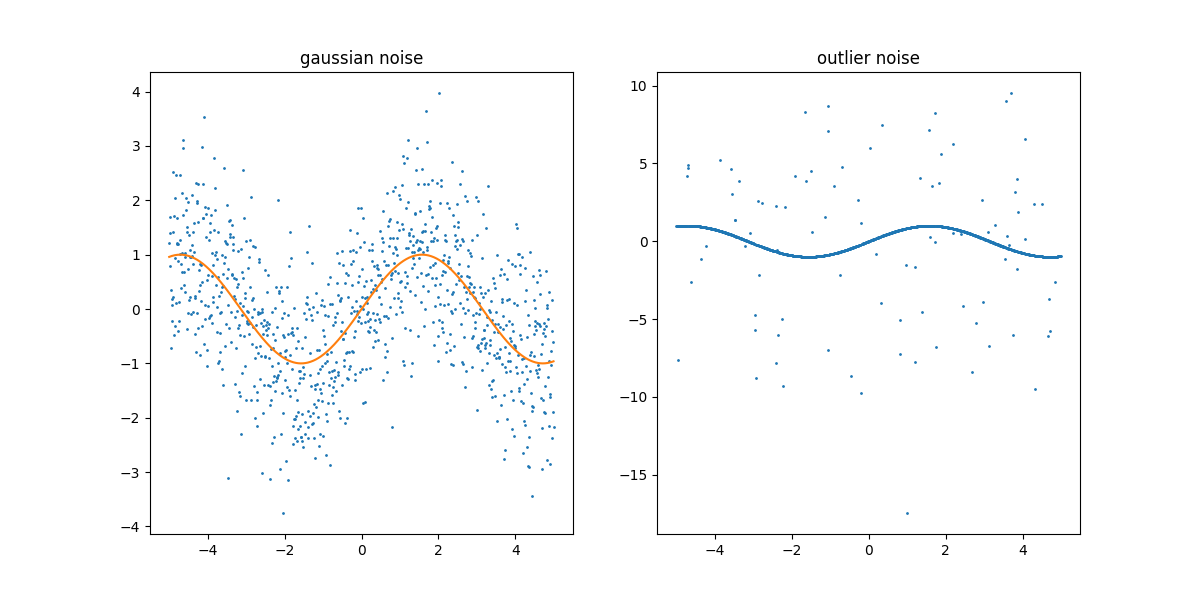
\includegraphics[keepaspectratio, scale=0.25]{assets/noise_example.png}
\end{center}
\end{frame}

\begin{frame}{Data Cleaning - Noise}

Noise model is used prove mathematically that some models are robust to noise. \\ However, not all of them are, e.g linear regression with L2 norm.

\end{frame}

\begin{frame}{Data Cleaning - Noise Reduction Techniques}

Several noise reduction techniques

\begin{itemize}
    \item Smoothing Techniques
    \item Regression Techniques
    \item Outlier Analysis
\end{itemize}
\end{frame}

\begin{frame}{Noise Reduction Techniques - Smoothing Techniques}
\begin{outline}
Let an attribute of data be \{ 1, 4, 5, 2, 14, 6, 20, 12, 6 \}
\begin{itemize}
    \item Step 1: Sort data \\
    \{ 1, 2, 4, 5, 6, 6, 12, 14, 20\}
    \item Step 2: Split data points into bins \\
    \{1, 2, 4\}, \{5, 6, 6\}, \{12, 14, 20\} 
    \item Step 3: Replace by Mean/Median or Boundaries \\ 
    Mean: \{2, 2, 2\}, \{6, 6, 6\}, \{15, 15, 15\} \\ 
    Median: \{2, 2, 2\}, \{6, 6, 6\}, \{14, 14, 14\}
\end{itemize}
\end{outline}
\end{frame}


\begin{frame}{Noise Reduction Techniques - Regression Techniques}
    \begin{columns}
    \begin{column}{0.5\textwidth}
        Density estimation by model robust to noise.
       \begin{itemize}
        \item Find the family of distributions suitable for data
        \item Find the best parameters of the distribution
        \item Confirm the validity of the assumption using statistical tests
        \item Replace data by samples from this distribution
    \end{itemize}
    \end{column}
    \begin{column}{0.5\textwidth}
        \begin{center}
        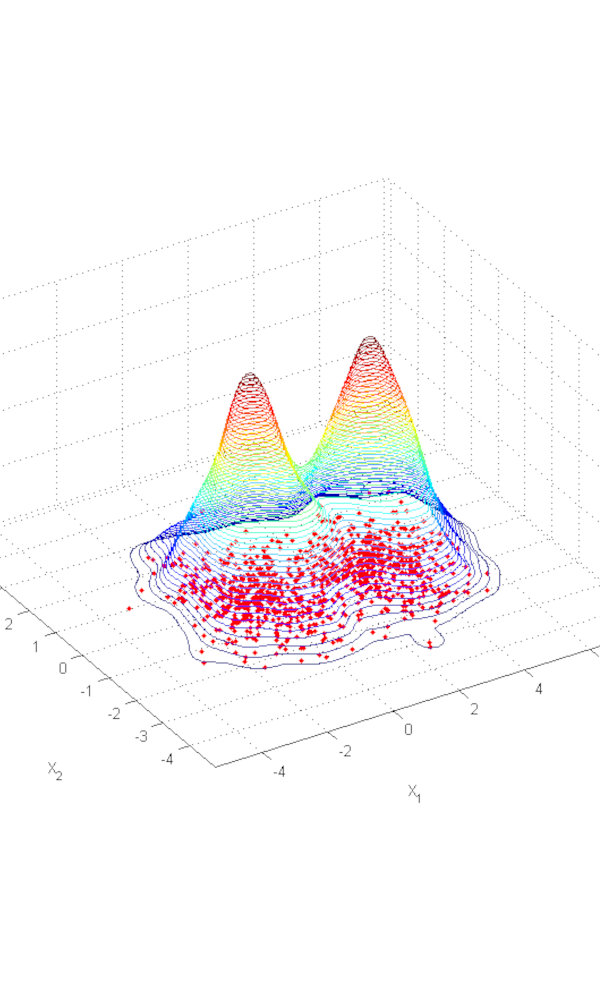
\includegraphics[width=0.7\textwidth]{assets/noise_regression.png}
        \end{center}
    \end{column}
    \end{columns}
\end{frame}

\begin{frame}{Noise Reduction Techniques - Outlier Analysis}
    Several techniques to detect outliers
    \begin{itemize}
        \item Inter-quartile Range Rule
        \item Local Outlier Factor
        \item Clustering
    \end{itemize}
\end{frame}


\subsubsection{Data Integration}
\begin{frame}{Data Integration - Motivation}

Data often come from multiple sources, there might be redundancy and correlation.

\end{frame}

\begin{frame}{Data Integration - Redundancy and Correlation Analysis}

Correlation Analysis

\begin{itemize}
    \item Nominal Data: $\chi^2$ correlation test (chi-square)
    \item Numeric Data: Correlation coefficient
\end{itemize}

Note: p-value = P(it is at least as extreme as the data | null hypothesis)

\end{frame}

\begin{frame}{Redundancy and Correlation Analysis - Nominal Data}
Let attribute $A$ has $c$ distinct values namely $a_1, a_2, ..., a_c$. attribute $B$ has $r$ distinct values namely $b_1, b_2, ..., b_r$.
\begin{exampleblock}{Pearson $\chi^2$ statistic}
    \begin{equation}
        \chi^2 = \sum_{i=1}^c \sum_{j=1}^r \frac{(o_{ij} - e_{ij})^2}{e_{ij}}
    \end{equation}
    where \\
    $o_{ij}  = count(A=a_i, B=b_j)$ is  the \emph{observed frequency} \\
    $e_{ij} = \frac{count(A=a_i) \times count(B=b_j)}{n}$ is the \emph{expected frequency}
\end{exampleblock}

Degree of freedom: $(c-1)(r-1)$ \\
Null hypothesis: $A$ and $B$ are independent
\end{frame}

\begin{frame}{Redundancy and Correlation Analysis - Numeric Data}
\begin{exampleblock}{Correlation coefficient}
\begin{equation*}
    r_{A, B} = \frac{cov(A, B)}{\sigma_A \sigma_B}
\end{equation*}
\end{exampleblock}

$r_{A, B} \in [-1, +1]$ \\
$r < 0 $ : negatively correlated \\
$r > 0 $ : positively correlated \\
$r = 0$ : independent

\end{frame}

\begin{frame}{Redundancy and Correlation Analysis - How to fix correlation?}
\begin{itemize}
    \item No correlation \\
        the ideal case
    \item Strongly correlated \\
        drop attribute (machine learning) \\
        train on masked input (deep learning) \\
    \item Weakly correlated \\ 
        Project to other space that those features are independent $\to$ \emph{Data Transformation}
\end{itemize}
\end{frame}

\subsubsection{Data Reduction}
\begin{frame}{Data Reduction - Motivation}

Sometimes, we want to reduce the data dimension or data size (numerosity) to

\begin{itemize}
    \item Reduce storage cost
    \item Reduce computational cost
\end{itemize}
\end{frame}

\begin{frame}{Dimensionality reduction}
    Reduce number of random variables
    \begin{itemize}
        \item Wavelet transform
        \item Principle component analysis
        \item Attribute subset selection
        \item Random projection
    \end{itemize}
\end{frame}

\begin{frame}{Dimensionality reduction - Wavelet transform}
    \begin{columns}
    \begin{column}{0.5\textwidth}
        Project a vector into wavelet basis.
        \begin{itemize}
            \item Generally better than Fourier transform
            \item There many families of wavelet - \emph{choose the family best suited for data}
        \end{itemize}
        
    \end{column}
    \begin{column}{0.5\textwidth}
        \begin{center}
            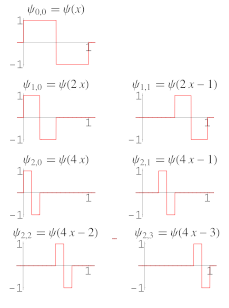
\includegraphics[width=0.8\textwidth]{assets/haar_wavelet.png}
        \end{center}
    \end{column}
    \end{columns}
\end{frame}


\begin{frame}{Dimensionality reduction - Principal component analysis}
    \begin{columns}
    \begin{column}{0.5\textwidth}
        Project a vector into PCA basis
        \begin{itemize}
            \item Maximize variance of data
        \end{itemize}
    \end{column}
    \begin{column}{0.5\textwidth}
        \begin{center}
            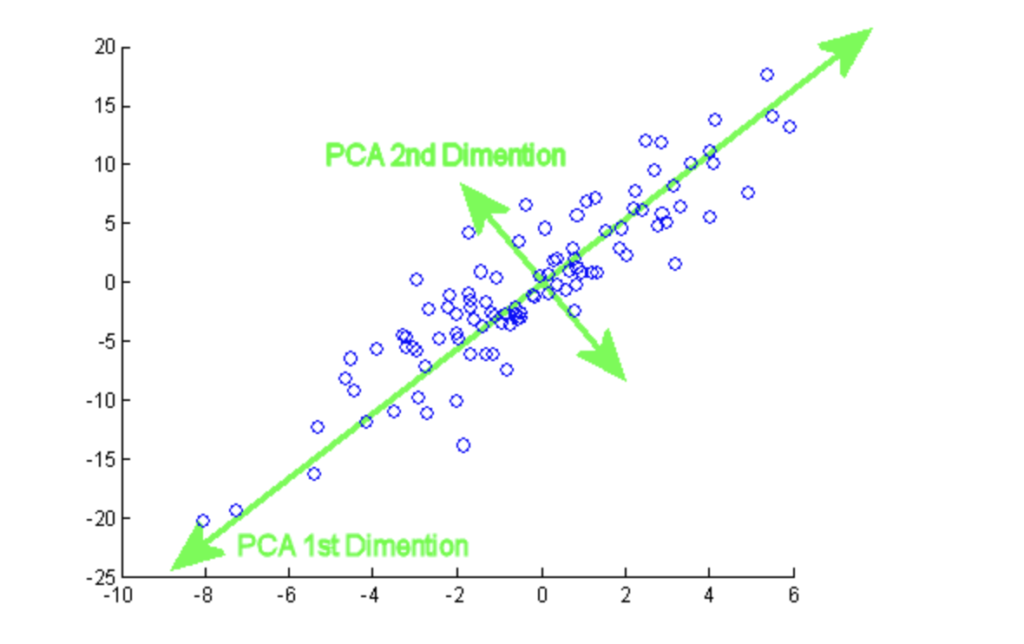
\includegraphics[width=1.0\textwidth]{assets/pca.png}
        \end{center}
    \end{column}
    \end{columns}
\end{frame}

\begin{frame}{Dimensionality reduction - Attribute subset selection}
    Greedy method to choose the best subset of attributes
    \begin{itemize}
        \item Stepwise forward selection
        \item Stepwise backward selection
        \item Decision tree induction
    \end{itemize}
\end{frame}

\begin{frame}{Dimensionality reduction - Attribute subset selection (cont)}
    \begin{center}
        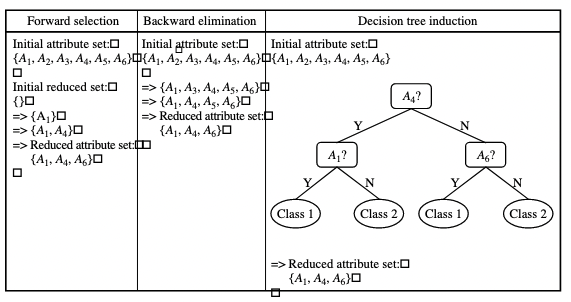
\includegraphics[width=1.0\textwidth]{assets/attr_subset_selection.png}
    \end{center}
\end{frame}

\begin{frame}{Dimensionality reduction - Random projection}
    \begin{columns}
    \begin{column}{0.5\textwidth}
        Based on \emph{JL lemma}, pair-wise distance distortion $0 < \epsilon < 1$, linear map $f: \mathbb{R}^d \to \mathbb{R}^k$ exists
        \begin{equation}
            k = \Omega ( \frac{\log n}{\epsilon^2} )
        \end{equation}
        Algorithm of $O(n)$ random projections
        
        \textbf{Projection:}
        \begin{itemize}
            \item Gaussian random projection $N(0, \frac{1}{k})$
            \item Sparse random projection
        \end{itemize}
    \end{column}
    \begin{column}{0.5\textwidth}
        \begin{center}
            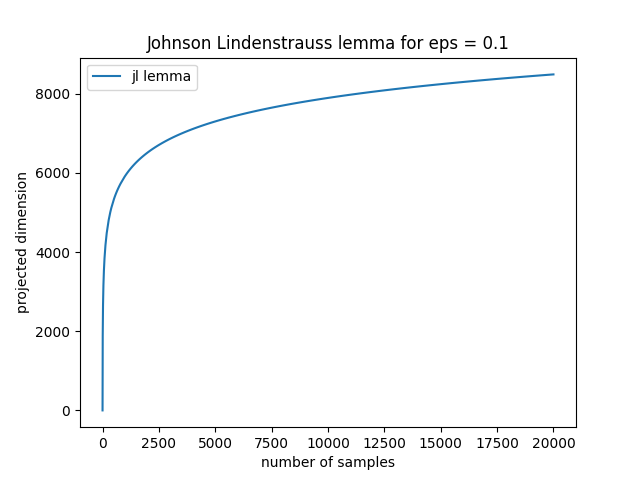
\includegraphics[width=1.0\textwidth]{assets/jl_lemma.png}
        \end{center}
    \end{column}
    \end{columns}
\end{frame}


\begin{frame}{Numerosity Reduction}
    Replace original data by a smaller representation

    \textbf{Parametric method} \\
    \begin{itemize}
        \item Estimate data by a model
        \item Save model parameters and outliers
    \end{itemize}
    \textbf{Non-parametric method}
    \begin{itemize}
        \item histogram
        \item clustering
        \item sampling (also in deep learning data augmentation)
    \end{itemize}
\end{frame}

\begin{frame}{Numerosity Reduction - Parametric method example}
    \textbf{Example} \\
    Give a set of data \{(1, 4, 0), (0, 3, 0), (7, 9, 0), (-1, 4, 2) \} \\
    Model: $z = 0$ \\
    Compressed data: \{(1, 4), (0, 3), (7, 9) \} \\
    Outliers: \{(-1, 4, 2)\} \\
\end{frame}

\begin{frame}{Numerosity Reduction - Non-parametric method example}
    \textbf{Histogram}
    \begin{itemize}
        \item divide domain into regions (lattice structure)
    \end{itemize}
    \textbf{Clustering}
    \begin{itemize}
        \item divide domain into regions (minimize loss)
    \end{itemize}
    \textbf{Sampling}
    \begin{itemize}
        \item random subsets of data
    \end{itemize}
\end{frame}

\begin{frame}{Numerosity Reduction - Non-parametric method example (cont)}
    \begin{columns}
    \begin{column}{0.5\textwidth}
         \begin{center}
            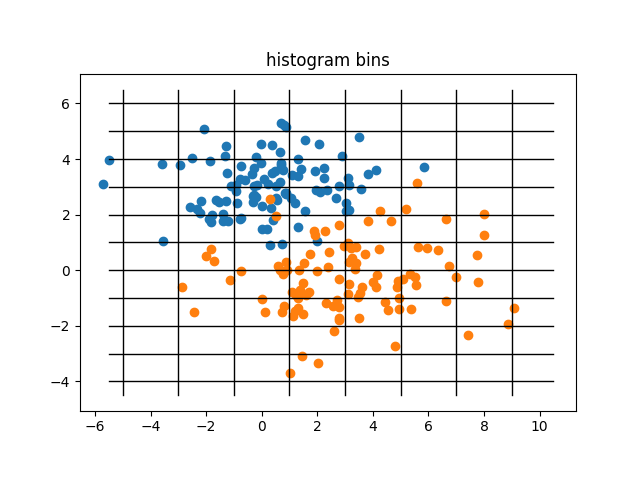
\includegraphics[width=1.0\textwidth]{assets/histogram_bins.png}
        \end{center}
    \end{column}
    \begin{column}{0.5\textwidth}
        \begin{center}
            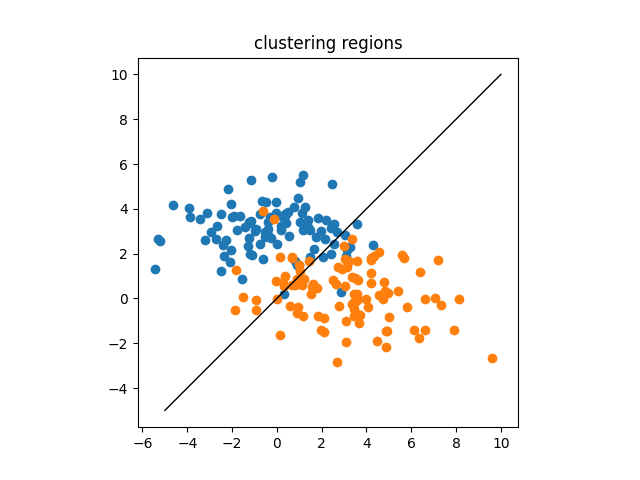
\includegraphics[width=1.0\textwidth]{assets/clustering_regions.png}
        \end{center}
    \end{column}
    \end{columns}
\end{frame}

\subsubsection{Data Discretization and Transformation}

\begin{frame}{Data Discretization and Transformation}

There many more discretization and transformation techniques \\

smoothing, feature construction, aggregation, normalization, discretization, concept hierarchy generation for nominal data (addr = unit + street), domain knowledge
\end{frame}